\documentclass{beamer}
\title{Read-Log-Update}
\subtitle{SOSP' 15}
\usetheme{CambridgeUS}
\usecolortheme{beaver}
%% \usepackage{makecell}
%% \usepackage{hyperref}
\usepackage[noend]{algpseudocode}
\usepackage{tabu}
\usepackage{kotex}
\usepackage{graphics}
\usepackage{booktabs}
\usepackage{listings}
\usepackage{local_dir}
\lstset{inputpath=\rlucode/Read-Log-Update/,
  basicstyle=\scriptsize,
  numbers=left,
  xleftmargin=10pt,
  tabsize=2,
  language=C,
}
\graphicspath{ {\rlufigure/Read-Log-Update/}}

\begin{document}

\author{
  \centering
  \begin{tabu}{c c c c}
    Alexander Matveev & Nir Shavit & Pascal Felber & Patrick Marlier\\
    \rowfont{\scriptsize}
    MIT & Tel-Aviv University & \multicolumn{2}{c}{University of Neuchatel}
  \end{tabu}
}

\begin{frame}
  \titlepage
  \begin{center}
    Chang-Hui Kim
  \end{center}
\end{frame}

%=================================================================

\section{The RLU Algorithm}

%=================================================================
%% needs some contents here!
%% first listing ideas
%% present simple graphic notatios
%% present basic idea with graphic
%% present Metadata

\begin{frame}[t]
  \frametitle{Basic Idea}
  RLU provides support for \textbf{multiple object updates in a single operation}
  by combining
  \begin{itemize}
  \item the quiescence mechanisim of RCU with a global clock.
  \item per thread object-level logs.
  \end{itemize}

\end{frame}

%=================================================================

\begin{frame}[t]
  \frametitle{Basic Idea}

  \begin{itemize}
  \item All operations read the global clock when they start. (into the local clock)
  \item Use the local clock to dereference the shared object.
  \item A write operation logs each object it modifies in a per thread write-log.
    \begin{itemize}
    \item write modifications are hidden from concurrent reads.
    \item avoid conflicts with concurrent writes.
    \end{itemize}
  \end{itemize}
  
\end{frame}

%=================================================================

\begin{frame}[t]
  \frametitle{Simple Graphic Notation}

  \begin{figure}[ht]
    \centering
    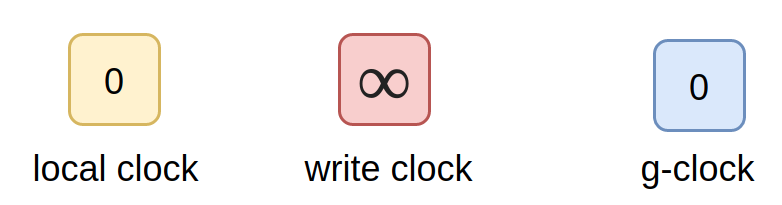
\includegraphics[width=0.7\textwidth]{simple_graphic.png}
  \end{figure}
  
\end{frame}

%=================================================================

\begin{frame}[t]
  \frametitle{Example}
  In this example, assume there is only one writer but multiple readers.
  \begin{figure}[ht]
    \centering
    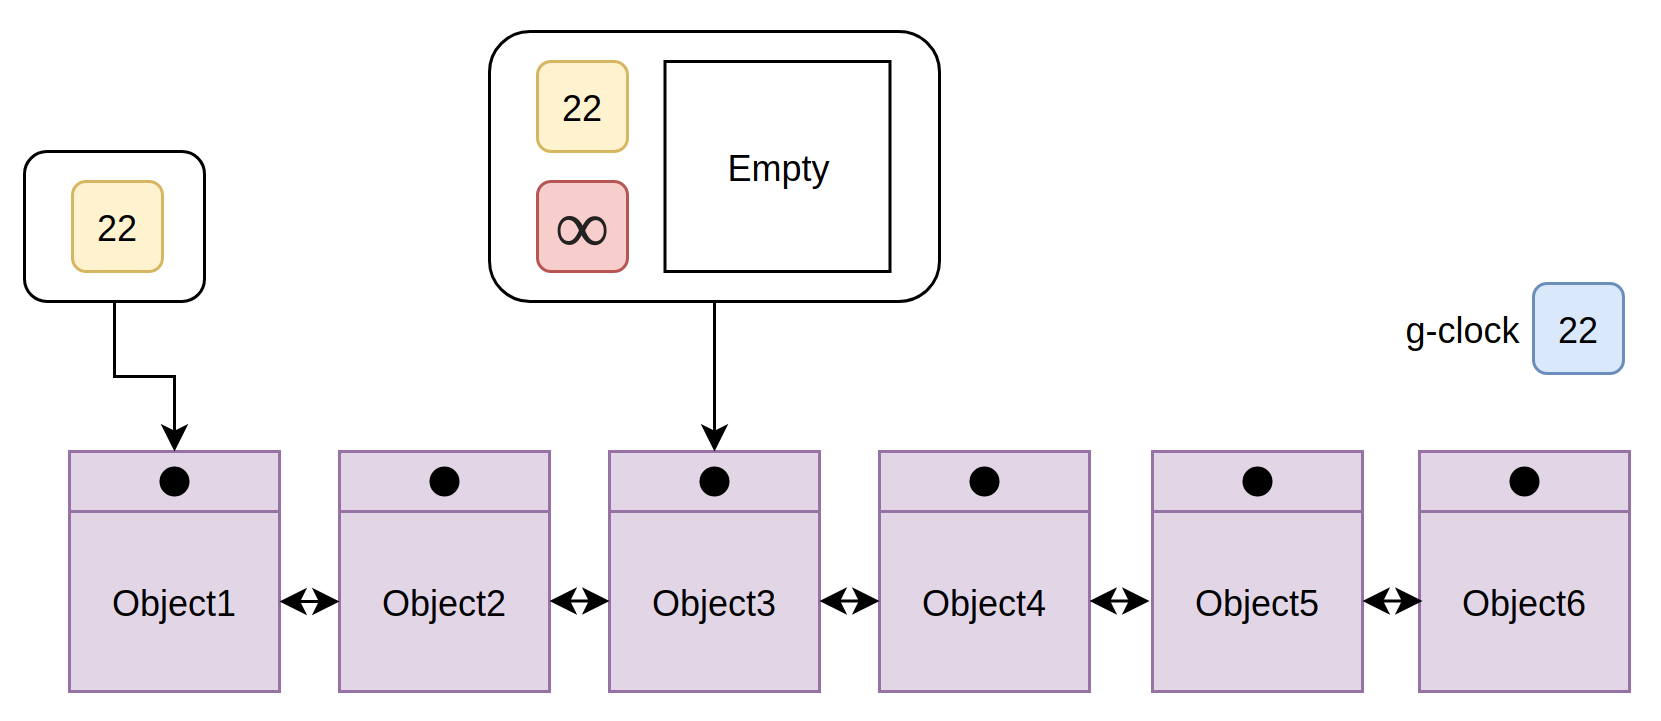
\includegraphics[width=0.7\textwidth]{start.png}
  \end{figure}

  \begin{itemize}
  \item All operations read the global clock when they start. (into local clock)
  \item Use local clock to dereference shared objects.\\
    (If $local\_clock \ge write\_clock$ then read log.) 

  \end{itemize}
  
\end{frame}

%=================================================================


\begin{frame}[t]
  \frametitle{Example}

  \begin{figure}[ht]
    \centering
    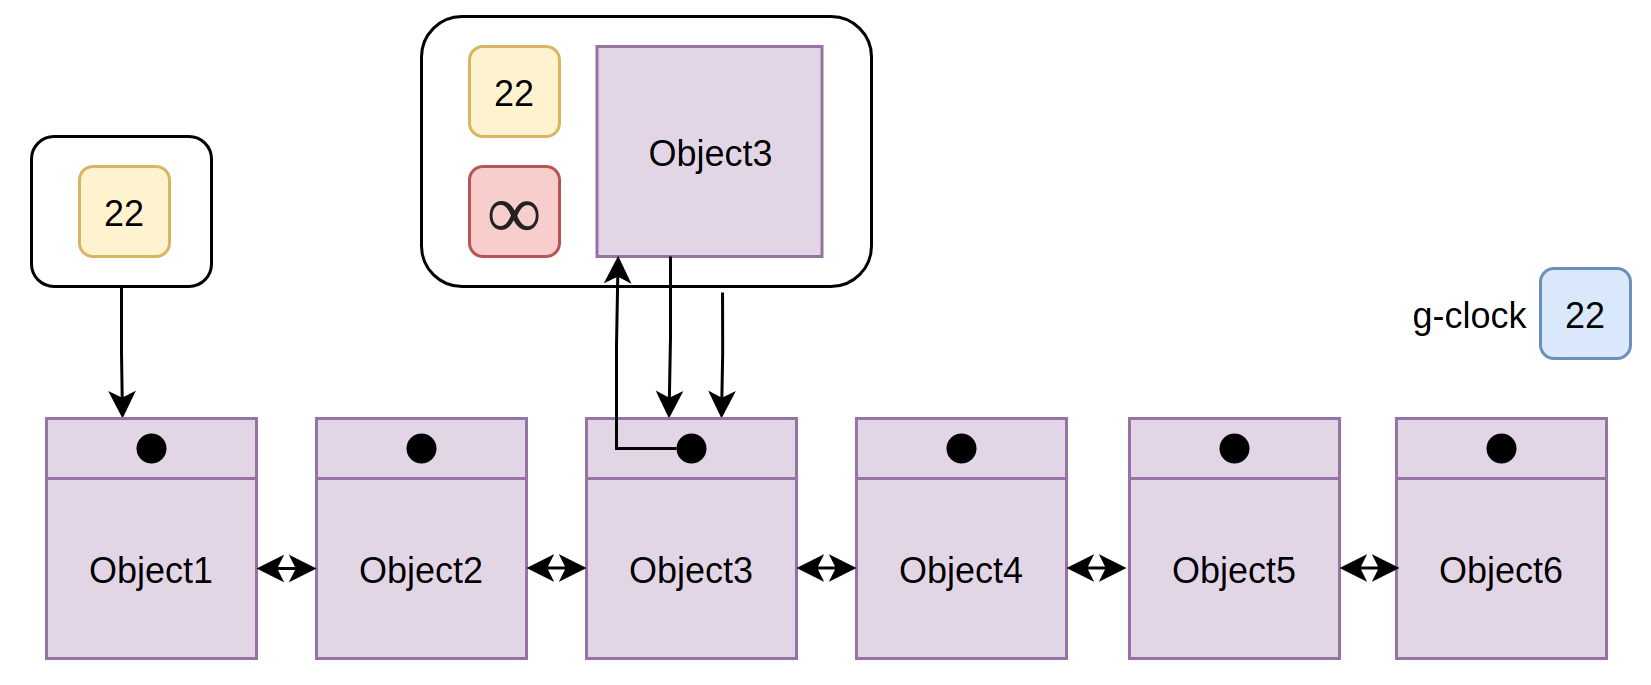
\includegraphics[width=0.7\textwidth]{lock_and_copy.png}
    \caption{Lock and Copy}
  \end{figure}

  The Writer
  \begin{enumerate}
  \item Initialize the write log header.
  \item Lock the object. (install the write log address into object header.)
  \item Copy the object into the write log.
  \end{enumerate}
  
\end{frame}

%=================================================================

\begin{frame}[t]
  \frametitle{Example}

  \begin{figure}[ht]
    \centering
    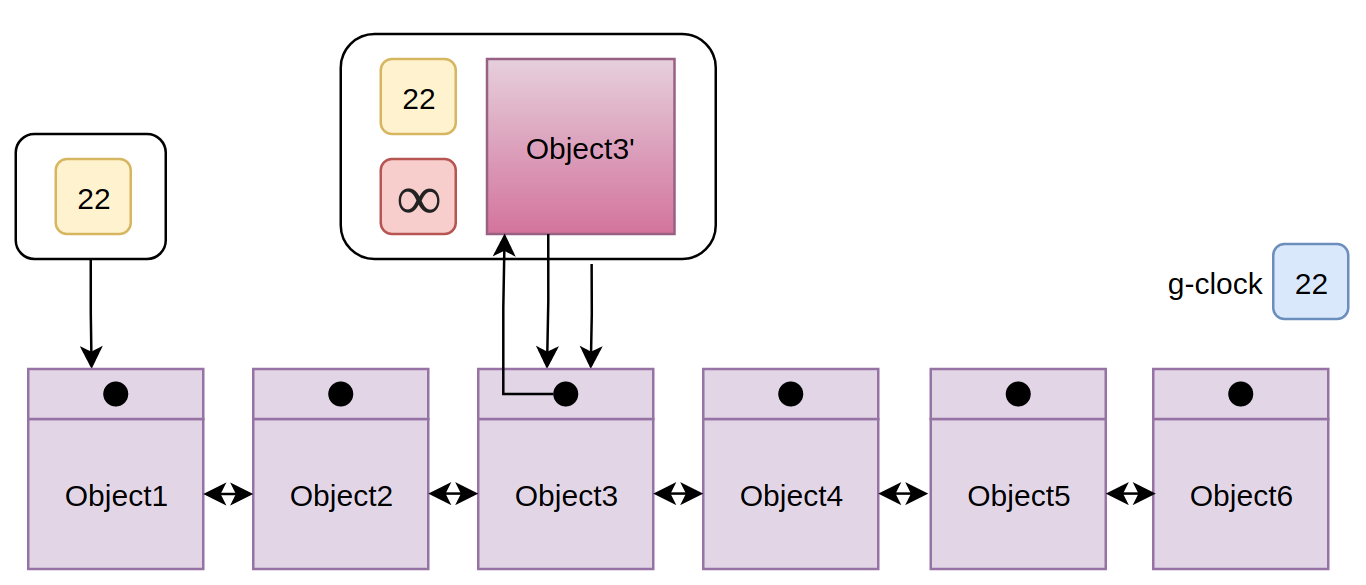
\includegraphics[width=0.7\textwidth]{write_on_log.png}
    \caption{Write on Log}
  \end{figure}

  \begin{itemize}
  \item The writer modifies the write log.
  \item No reader can read that log cause the write clock is infinity.
  \end{itemize}
  
\end{frame}

%=================================================================

\begin{frame}[t]
  \frametitle{Example}

  \begin{figure}[ht]
    \centering
    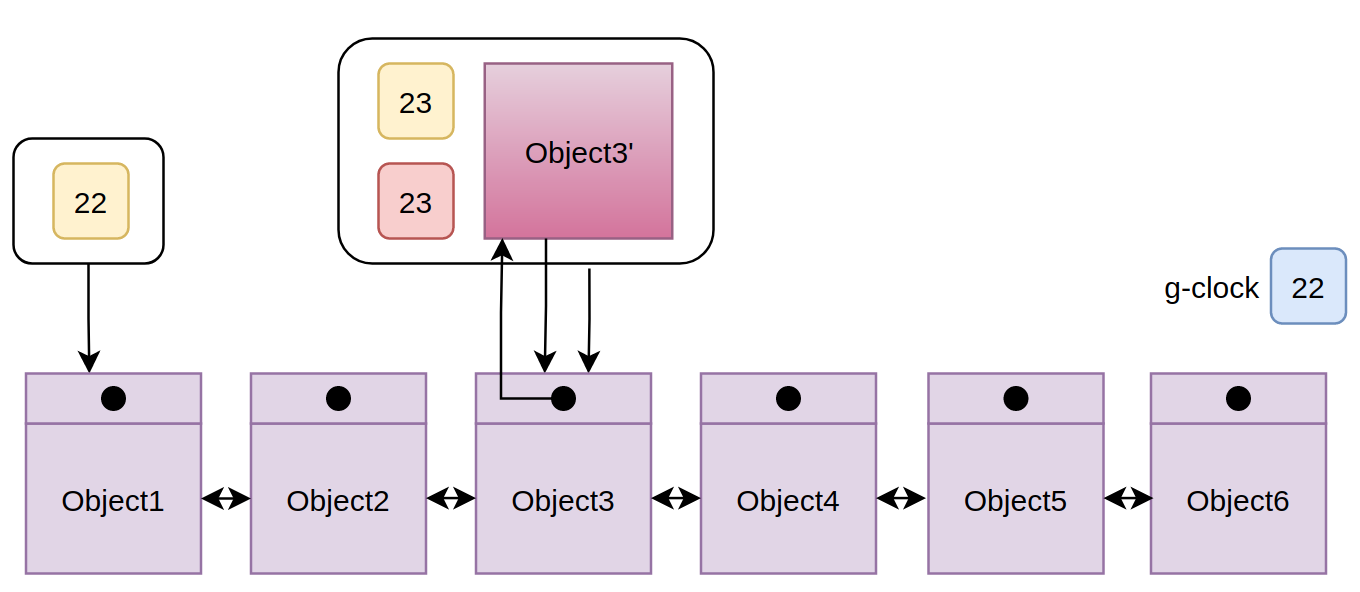
\includegraphics[width=0.7\textwidth]{commit_1.png}
    \caption{Commit --- 1}
  \end{figure}

  \begin{itemize}
  \item The writer calculates the next global clock and sets that value into local and write clock.
  \item No others can see the write log yet.
  \end{itemize}
  
\end{frame}

%=================================================================

\begin{frame}[t]
  \frametitle{Example}

  \begin{figure}[ht]
    \centering
    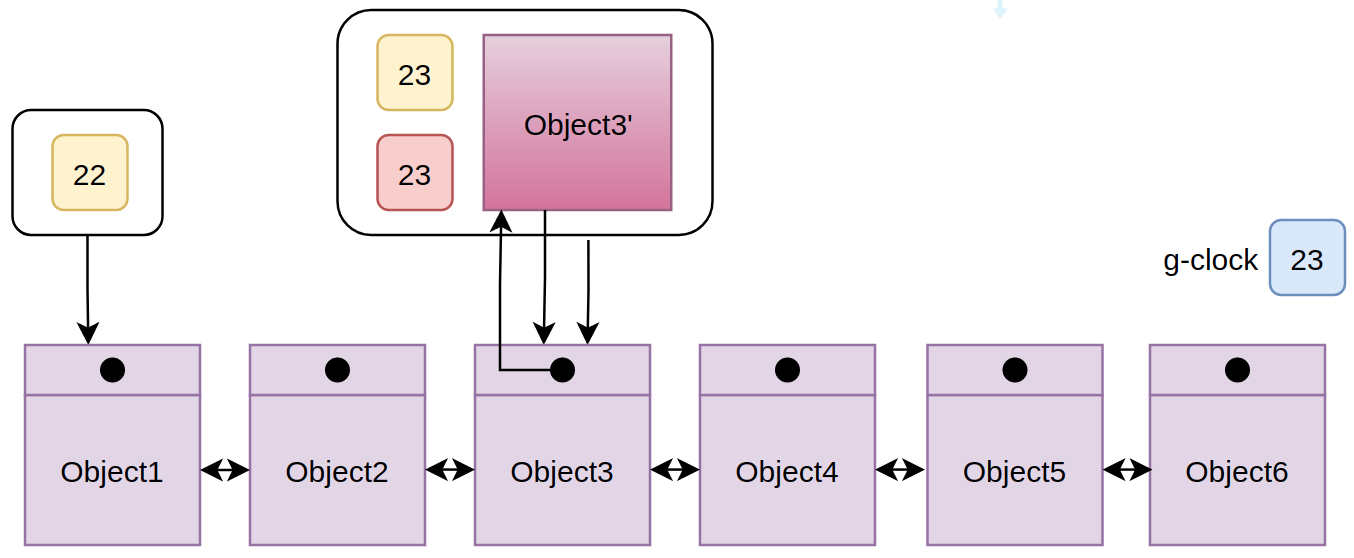
\includegraphics[width=0.7\textwidth]{commit_2.png}
    \caption{Commit --- 2}
  \end{figure}

  \begin{itemize}
  \item The writer increases the global clock by one. (final step of commit.)
  \item That Atomic operation (increase the global clock) splits the old and the new operation.
  \end{itemize}
  
\end{frame}

%=================================================================

\begin{frame}[t]
  \frametitle{Example}

  \begin{figure}[ht]
    \centering
    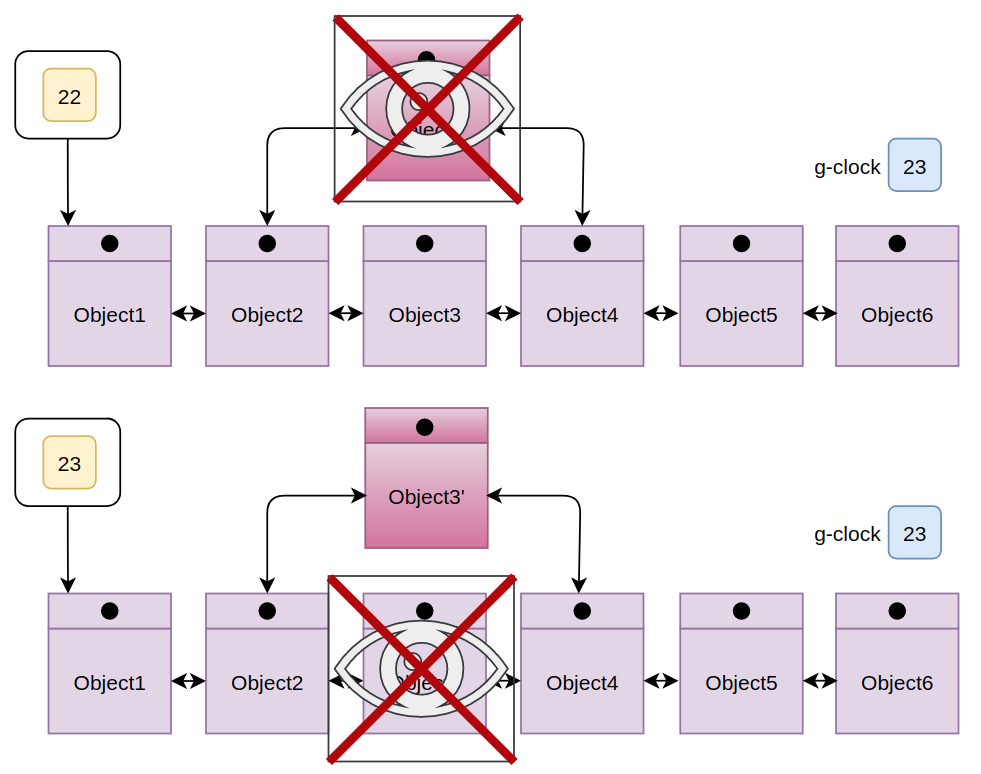
\includegraphics[width=0.6\textwidth]{read_view.png}
    \caption{Read Side Memory View}
  \end{figure}
  
\end{frame}

%=================================================================

\begin{frame}[t]
  \frametitle{Example}

  \begin{figure}[ht]
    \centering
    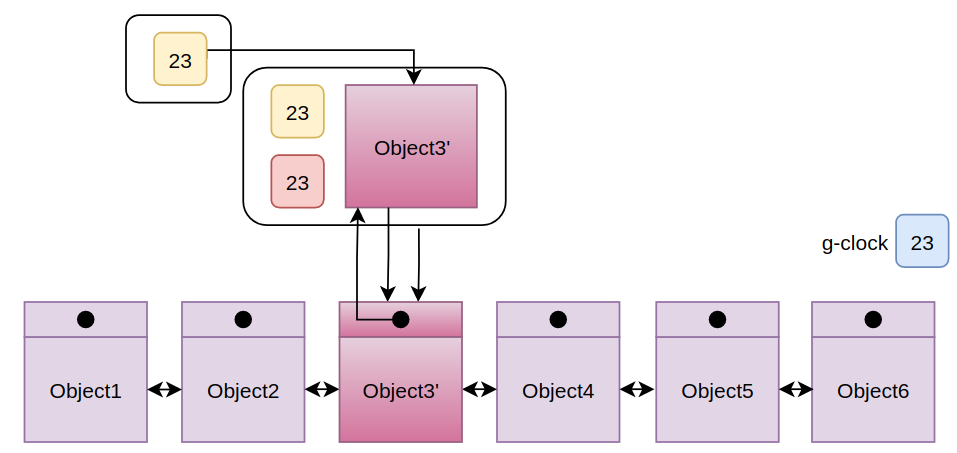
\includegraphics[width=0.7\textwidth]{steal.png}
    \caption{Steal}
  \end{figure}

  \begin{itemize}
  \item Readers who have the local clock is greater or equal to the write clock
    can see the write log. (steal)
  \item The writer waits for the old operations to finish and then ``write back''
    to the actual object.
  \end{itemize}
  
\end{frame}

%=================================================================

\begin{frame}[t]
  \frametitle{Example}

  \begin{figure}[t]
    \centering
    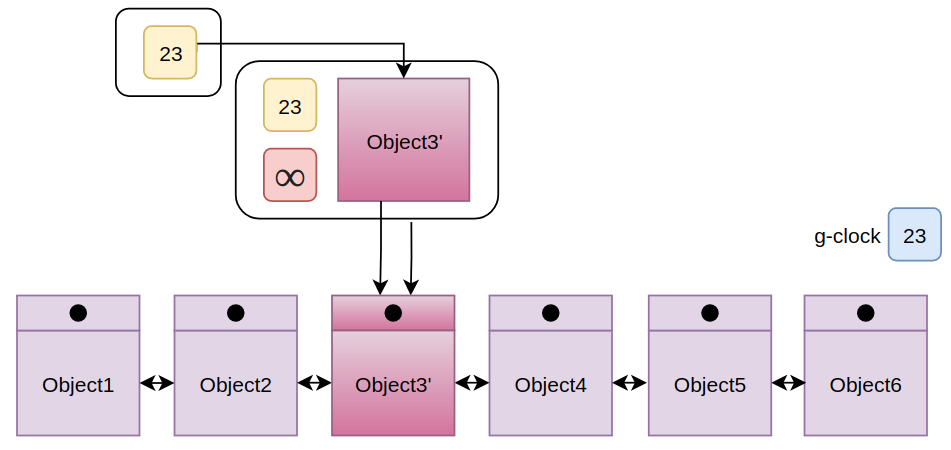
\includegraphics[width=0.7\textwidth]{unlock.png}
    \caption{What about that thief?}
  \end{figure}

  The writer
  \begin{itemize}
  \item unlocks the actual object. (assign \texttt{NULL} into the actual object header.)
  \item sets an infinite value into the write clock.
  \end{itemize}
  
\end{frame}

%=================================================================

\begin{frame}[t]
  \frametitle{RLU Metadata}
  \begin{columns}
    \begin{column}{.5\textwidth}
      \emph{Global.}
      \begin{itemize}
      \item Global Clock
      \item Global Array of Threads
      \end{itemize}
    \end{column}

    \begin{column}{.5\textwidth}
      \begin{figure}[ht]
        \centering
        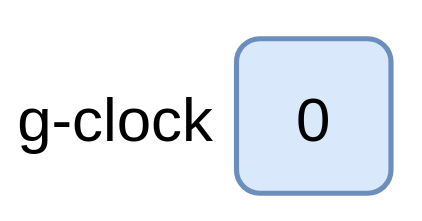
\includegraphics[width=0.5\textwidth]{g_clock.png}
        \caption{Global Clock}
      \end{figure}
    \end{column}
  \end{columns}
  
\end{frame}

%=================================================================

\begin{frame}[t]
  \frametitle{RLU Metadata}

  \begin{columns}
    \begin{column}{.5\textwidth}
      \emph{Object.}
      \begin{itemize}
      \item pointer that points to the object copy.\\
        if pointer is \texttt{NULL} then
        \begin{enumerate}
        \item no copy object.
        \item this object is \textbf{unlocked}.
        \end{enumerate}
      \end{itemize}
    \end{column}

    \begin{column}{.5\textwidth}
      \begin{figure}[ht]
        \centering
        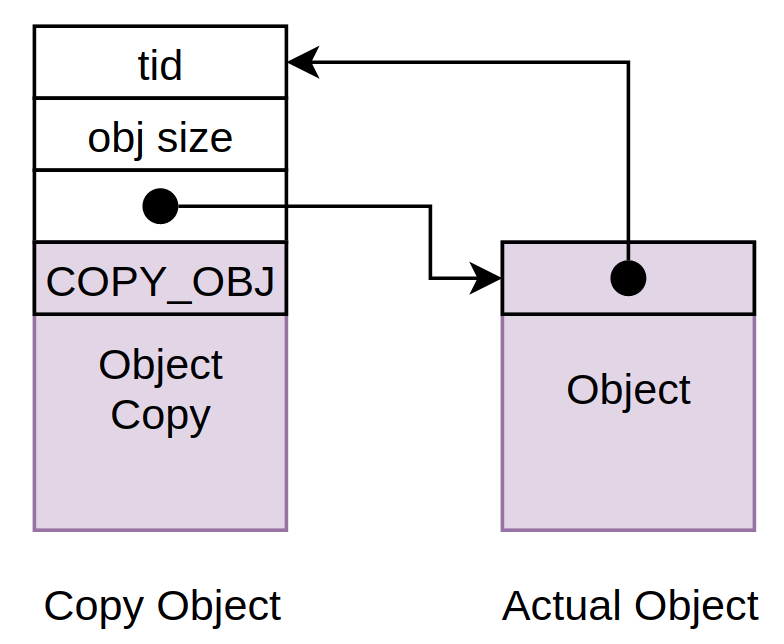
\includegraphics[width=\textwidth]{Object.png}
        \caption{RLU Object}
      \end{figure}
    \end{column}
  \end{columns}
  
\end{frame}

%=================================================================

\begin{frame}[t]
  \frametitle{RLU Metadata}

  \begin{columns}
    \begin{column}{.5\textwidth}
      \emph{Object Copy.}
      \begin{itemize}
      \item thread identifier
      \item object size
      \item pointer to the actual object
      \item a special pointer value that indicates this
        object is copy. (\texttt{COPY\_OBJ})
      \end{itemize}
    \end{column}

    \begin{column}{.5\textwidth}
      \begin{figure}[ht]
        \centering
        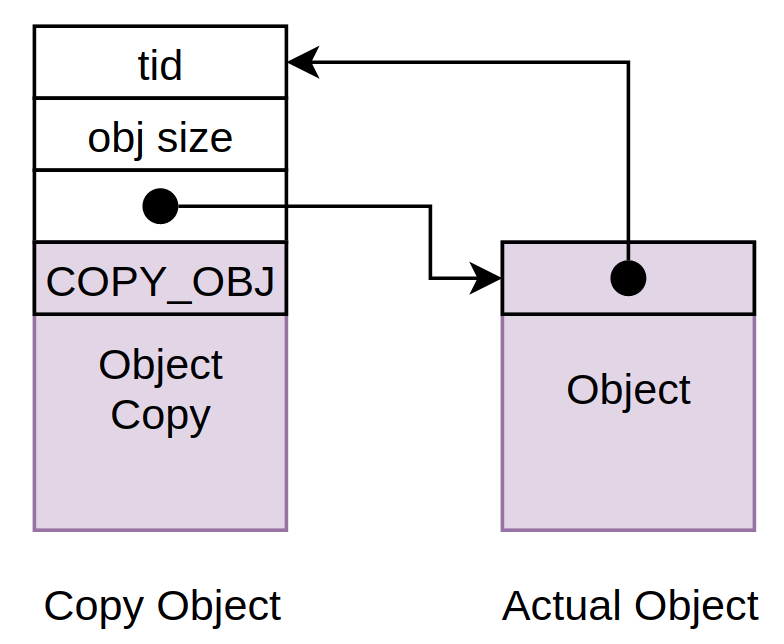
\includegraphics[width=\textwidth]{Object.png}
        \caption{RLU Object}
      \end{figure}
    \end{column}
  \end{columns}
  
\end{frame}

%=================================================================

\begin{frame}[t]
  \frametitle{RLU Metadata}

  \emph{Write Log.}\\
  has multiple Copy Objects.

  \begin{figure}[ht]
    \centering
    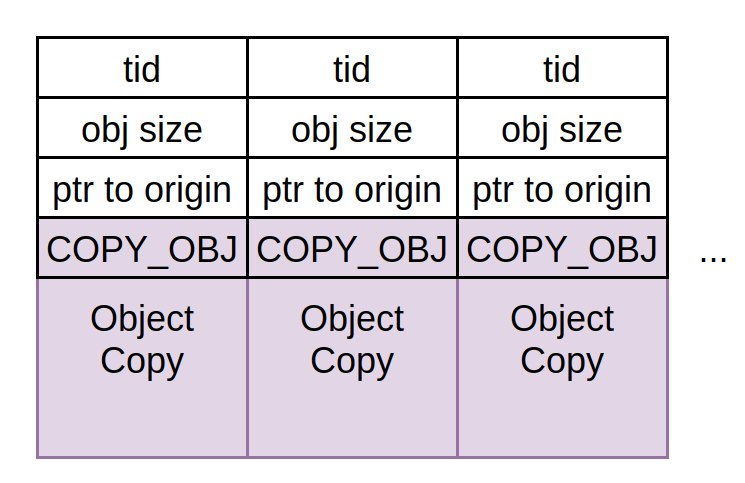
\includegraphics[width=.6\textwidth]{write_log.png}
    \caption{Write Log}
  \end{figure}
  
\end{frame}

%=================================================================

\begin{frame}[t]
  \frametitle{RLU Metadata}

  \begin{columns}
    \begin{column}{.3\textwidth}
      \emph{Threads.}
      \begin{itemize}
      \item two write logs
      \item local clock
      \item write clock
      \item run counter
      \end{itemize}
    \end{column}

    \begin{column}{.7\textwidth}
      \begin{figure}[ht]
        \centering
        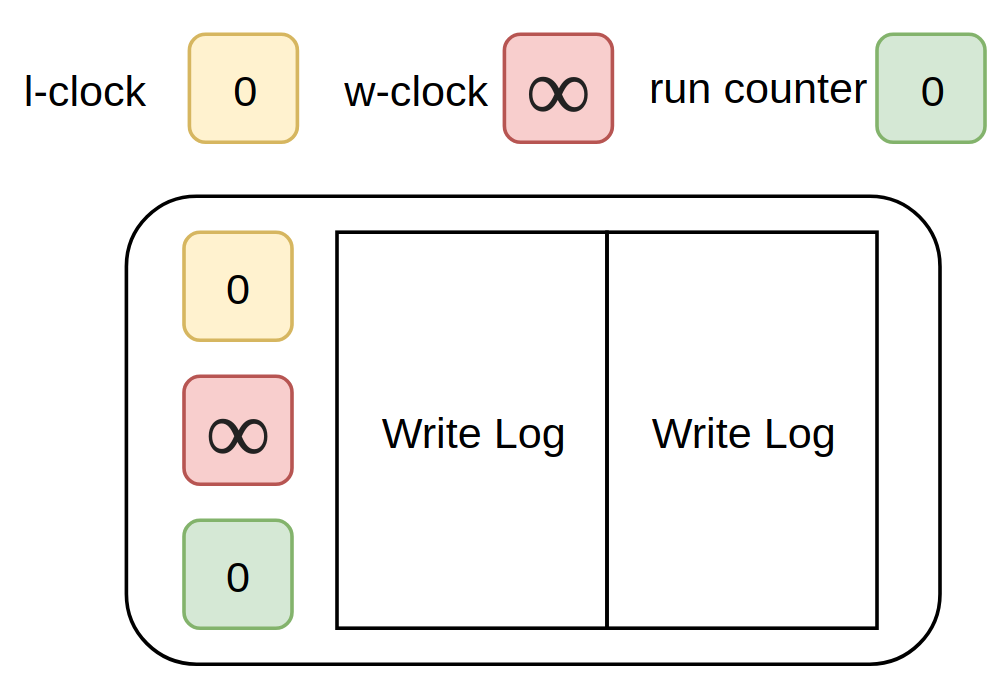
\includegraphics[width=\textwidth]{thread.png}
        \caption{RLU Thread}
      \end{figure}
    \end{column}
  \end{columns}
  
\end{frame}

%=================================================================

\begin{frame}[t]
  \frametitle{Fine-grained Locking Using RLU}
  In RLU
  \begin{itemize}
  \item each object that a writer modifies is logged and locked.
    \begin{enumerate}
    \item traverse the data structure.
    \item lock and copy the target data.
    \item if the locking fails, then the operation restarts.
    \end{enumerate}
  \end{itemize}
  
\end{frame}

%=================================================================

\begin{frame}[t]
  \frametitle{Pseudo Code}

    \footnotesize{
    \begin{algorithmic}
      \Function{RLU\_TRY\_LOCK}{ctx, obj}
      \State ctx.is-writer $\leftarrow$ \textbf{true} \Comment{this thread is writer}
      \State obj $\leftarrow$ GET\_ACTUAL(obj)
      \State ptr-copy $\leftarrow$ GET\_COPY(obj)

      \If {$\neg$IS\_UNLOCKED(ptr-copy)}
      \State thr-id $\leftarrow$ GET\_THREAD\_ID(ptr-copy)
      \If {thr-id $=$ ctx.thr-id}
      \State \Return ptr-copy
      \EndIf

      \State RLU\_ABORT(ctx) \Comment{Retry RLU Section}
      \EndIf

      \State obj-header.thr-id $\leftarrow$ ctx.thr-id
      \State obj-header.obj $\leftarrow$ obj
      \State obj-header.obj-size $\leftarrow$ SIZEOF(obj)
      \State ptr-copy $\leftarrow$ LOG\_APPEND(ctx.write-log, obj-header)

      \If {$\neg$TRY\_LOCK(obj, ptr-copy)} \Comment{Try to install copy (CAS)}
      \State RLU\_ABORT(ctx)
      \EndIf
      \State LOG\_APPEND(ctx.write-log, obj) \Comment{Locked $\Rightarrow$ copy object}
      \State \Return ptr-copy
      \EndFunction
    \end{algorithmic}
  }
  
\end{frame}

%=================================================================

\begin{frame}[t]
  \frametitle{Pseudo Code}
  
  \footnotesize{
    \begin{algorithmic}
      \Function{RLU\_COMPARE\_OBJ}{ctx, obj1, obj2}
      \State \Return GET\_ACTUAL(obj1) $=$ GET\_ACTUAL(obj2)
      \EndFunction

    \end{algorithmic}

    \begin{algorithmic}
      \Function{RLU\_ASSIGN\_PTR}{ctx, handle, obj}
      \State *handle $\leftarrow$ GET\_ACTUAL(obj)
      \EndFunction
    \end{algorithmic}
  }

\end{frame}

%=================================================================

\begin{frame}[t]
  \frametitle{Pseudo Code}

  \footnotesize{
    \begin{algorithmic}
      \Function{RLU\_DEREFERENCE}{ctx, obj}
      \State ptr-copy $\leftarrow$ GET\_COPY(obj) \Comment{Get copy pointer}

      \If {IS\_UNLOCKED(ptr-obj)}
      \State \Return obj
      \EndIf

      \If {IS\_COPY(ptr-obj)}
      \State \Return obj
      \EndIf

      \State thr-id $\leftarrow$ GET\_THREAD\_ID(ptr-copy)
      \If {thr-id $=$ ctx.thr-id}
      \State \Return ptr-copy
      \EndIf

      \State other-ctx $\leftarrow$ GET\_CTX(thr-id) \Comment{Get owner thread ctx}
      \If {other-ctx.write-clock $\le$ ctx.local-clock}
      \State \Return ptr-copy
      \EndIf

      \State \Return obj
      \EndFunction
    \end{algorithmic}
  }

\end{frame}

%=================================================================

\begin{frame}[t]
  \frametitle{Pseudo Code}

    \footnotesize{
    \begin{algorithmic}
      \Function{RLU\_SYNCHRONIZE}{ctx} \Comment{Capture current state}
      \For{thr-id $\in$ active-threads}
      \State other $\leftarrow$ GET\_CTX(thr-id)
      \State ctx.sync-cnts[thr-id] $\leftarrow$ other.run-cnt
      \EndFor

      \For{thr-id $\in$ active-thread} \Comment{Wating for old opeartions}
      \While{\textbf{true}}
      \If {ctx.sync-cnts[thr-id] is even}
      \State \textbf{break}
      \EndIf

      \State other $\leftarrow$ GET\_CTX(thr-id)
      \If {ctx.sync-cnts[thr-id] $\ne$ other.run-cnt}
      \State \textbf{break}
      \EndIf

      \If {ctx.write-clock $\le$ other.local-clock}
      \State \textbf{break}
      \EndIf
      \EndWhile
      \EndFor

      \EndFunction
    \end{algorithmic}
  }

\end{frame}

%=================================================================

\begin{frame}[t]
  \frametitle{Pseudo Code}
  \footnotesize{
  \begin{algorithmic}
    \Function{RLU\_ABORT}{ctx, obj}
    \State ctx.run-cnt $\leftarrow$ ctx.run-cnt + 1 \Comment{set inactive}
    \If {ctx.is-writer}
    \State RLU\_UNLOCK\_WRITE\_LOG(ctx) \Comment{Unlock}
    \State RETRY
    \EndIf
    \EndFunction
  \end{algorithmic}
  }

\end{frame}

%=================================================================

\begin{frame}[t]
  \frametitle{Pseudo Code}

  \footnotesize{
    \begin{algorithmic}
      \Function{RLU\_READER\_LOCK}{ctx}
      \State ctx.is-writer $\leftarrow$ \textbf{false}
      \State ctx.run-cnt $\leftarrow$ ctx.run-cnt + 1 \Comment{Set active}
      \State \textbf{memory fence}
      \State ctx.local-clock $\leftarrow$ global-clock \Comment{Record global clock}
      \EndFunction
    \end{algorithmic}

    \begin{algorithmic}
      \Function{RLU\_READER\_UNLOCK}{ctx}
      \State ctx.run-cnt $\leftarrow$ ctx.run-cnt + 1 \Comment{Set inactive}
      \If{ctx.is-writer}
      \State RLU\_COMMIT\_WRITE\_LOG(ctx) \Comment{Write updates}
      \EndIf
      \EndFunction
    \end{algorithmic}
  }

\end{frame}

%=================================================================

\begin{frame}[t]
  \frametitle{Pseudo Code}
  
    \footnotesize{
    \begin{algorithmic}
      \Function{RLU\_COMMIT\_WRITE\_LOG}{ctx}
      \State ctx.write-clock $\leftarrow$ global-clock + 1 \Comment{Order is important}
      \State FETCH\_AND\_ADD(global)
      \State RLU\_SYNCHRONIZE(ctx)
      \State RLU\_WRITEBACK\_WRITE\_LOG(ctx)
      \State ctx.write-clock $\leftarrow \infty$ \Comment{Disable stealing}
      \State RLU\_SWAP\_WRITE\_LOGS(ctx) \Comment{Quiesce write-log}
      \EndFunction
    \end{algorithmic}
  }

\end{frame}

%=================================================================

\begin{frame}[t]
  \frametitle{Pseudo Code}
  \footnotesize{
  \begin{algorithmic}
    \Function{RLU\_SWAP\_WRITE\_LOGS}{ctx}
    \State ptr-write-log $\leftarrow$ ctx.write-log-quiesce \Comment{Swap pointers}
    \State ctx.write-log-quiesce $\leftarrow$ ctx.write-log
    \State ctx.write-log $\leftarrow$ ptr-write-log
    \EndFunction
  \end{algorithmic}
  }

  \begin{itemize}
  \item Within \texttt{RLU\_COMMIT\_WRITE\_LOG}, \texttt{RLU\_SYNCHRONIZE} has called.\\
    $\rightarrow$ So there are no more thieves on the previous write log.
  \end{itemize}

  % need graphic here!!! why need two write logs.
  % why don't have to wait the steal threads.
  
\end{frame}

%=================================================================

\begin{frame}[t]
  \frametitle{Correctness}
  The key for correctness is to ensure that

  \begin{center}
    \emph{RLU protected sections always execute on a consistent memory view}.
  \end{center}

\end{frame}

%=================================================================

\begin{frame}[t]
  \frametitle{Correctness}

  On Commit an writer increments the global clock.
  \begin{itemize}
  \item ``splits'' all concurrent RLU sections into \emph{old} and \emph{new}.\\
    (depends on local clock)
  \item \texttt{RLU\_DEREFERENCE} ensures that
    \begin{itemize}
    \item new sections can only read the object copy. (stealing)
    \item old sections can only read the actual object.
    \end{itemize}
  \end{itemize}

  \begin{center}
    After old sections complete (via synchronize call), no other thread can read
    the actual memory of modified object. (now ``write back'' is safe)
  \end{center}

\end{frame}

%=================================================================

\begin{frame}[t]
  \frametitle{Correctness}
  After the write-back of RLU writer, the write-log cannot be used immediately. (cause of thieves!)\\
  So,
  \begin{enumerate}
  \item swaps the current write-log \emph{$L_1$} with a new write-log \emph{$L_2$}.
  \item only after next commits and completes its RLU synchronize call for
    \begin{itemize}
    \item write back \emph{$L_2$} on actual object.
    \item \emph{$L_1$} thieves!
    \end{itemize}
  \item after this RLU synchronize call completes, it is safe to reuse the \emph{$L_1$}.
  \end{enumerate}
\end{frame}

%=================================================================

\begin{frame}[t]
  \frametitle{Correctness}
  Finally, to avoid write-write conflicts between writers, each RLU writer locks each object it wants to modify.
  
\end{frame}

%=================================================================

\begin{frame}[t]
  \frametitle{RLU Deferring}
  Each RLU writer must execute one RLU synchronize call during the process of commit.
  \begin{itemize}
  \item usually it becomes expensive when operations are short and fast.
  \end{itemize}

  \begin{center}
    So, defer the RLU synchronize call!
  \end{center}
  
\end{frame}

%=================================================================

\begin{frame}[t]
  \frametitle{RLU Deferring}

  On commit,
  \begin{enumerate}
  \item saves the current write-log.
  \item generates a new log for the next write opeartion.
  \end{enumerate}

  \begin{itemize}
  \item the write-log is still invisible.
  \item the actual object is still locked.
  \end{itemize}
  
\end{frame}

%=================================================================

\begin{frame}[t]
  \frametitle{RLU Deferring}

  The RLU synchronize call is actually only necessary when
  a writer tries to lock an object that is already locked.\\

  The writer sends a ``sync request'' to the conflicting thread to force it to
  \begin{enumerate}
  \item increment the global clock
  \item execute RLU synchronize
  \item write back
  \item unlock
  \end{enumerate}
  
\end{frame}

%=================================================================

\begin{frame}[t]
  \frametitle{RLU Deferring}

  Pros
  \begin{itemize}
  \item reduces the amount of RLU synchronize calls (only for W/W conflict)
  \item reduces the contention on the global clock
  \item defers the stealing process to a later time\\
    $\rightarrow$ reduce readers cache misses.
  \end{itemize}
  
\end{frame}

%=================================================================

\begin{frame}[t]
  \frametitle{RLU Deferring}

  Cons
  \begin{itemize}
  \item a lagging thread may delay other threads that wait for a sync response from this thread.\\
    $\rightarrow$ sync and write back instead of the lagging thread.
  \item requires to define specific sync points in the code where it is critical to see the most recent updates.
  \end{itemize}
  % 아니 그럼 write 하고 나서 다시 시스템에 들어왔는데 내가 수정한 부분이 반영이 안되어 있다는 거는 어떻게 처리할 것인지?
  
\end{frame}

%=================================================================

\section{Evaluation}

%=================================================================

% 자료구조 특성, 실험 환경, 테스트 방법, 결과 해석, 주장

\subsection{Micro-Benchmarks}

%=================================================================

\begin{frame}[t]
  \frametitle{Linked List}

  \begin{itemize}
  \item vs
    \begin{itemize}
    \item Harris-Michael (with memory leak)
    \item Harris-Michael (with hazard pointer)
    \item URCU
    \end{itemize}
  \item enviroment
    \begin{itemize}
    \item 16-way Intel Core i7-5960X 3GHz 8-core chip\\
      (with 2 hardware hyperthreads per core)
    \item Linux 3.13 x86\_64
    \item GCC 4.8.2 C/C++ compiler
    \end{itemize}
  \end{itemize}

\end{frame}

%=================================================================

\begin{frame}[t]
  \frametitle{Linked List}

  \begin{figure}[ht]
    \centering
    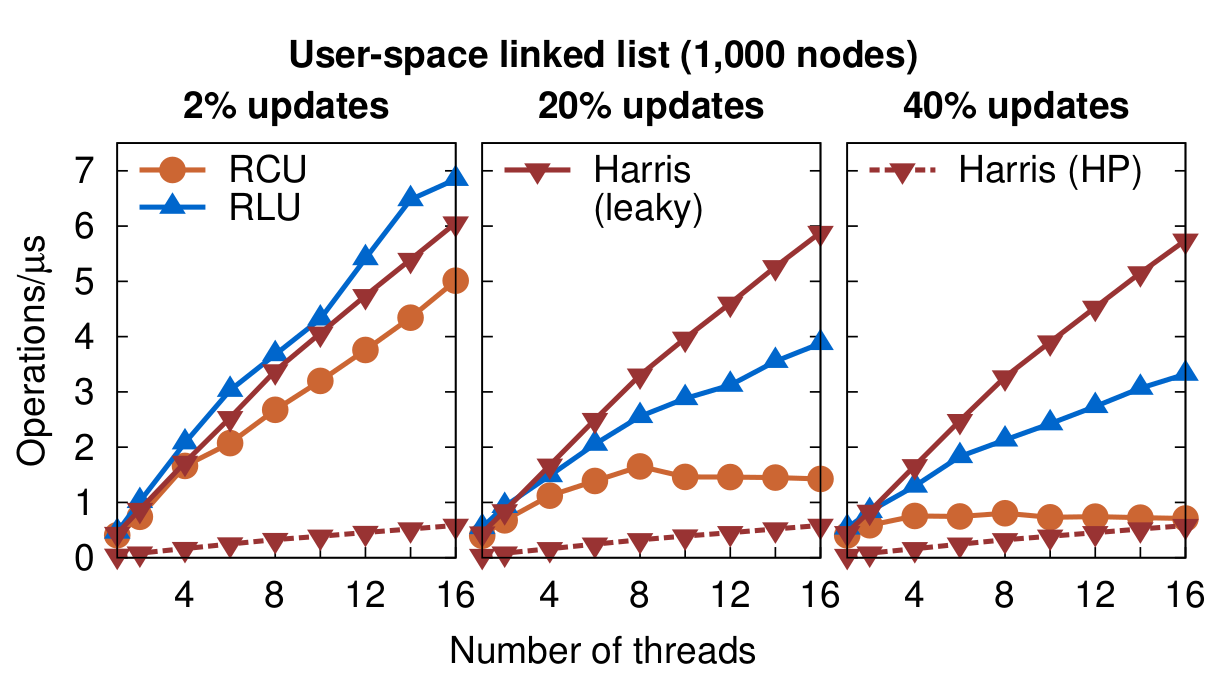
\includegraphics[width=0.8\textwidth]{user-space-linked-list-bench.png}
  \end{figure}

  \begin{itemize}
  \item hazard pointer uses memory fence on every dereference.
  \item RCU writers execute serially.
  \end{itemize}
  
\end{frame}

%=================================================================

\begin{frame}[t]
  \frametitle{Hash Table}
  A simple hash table data-structure that uses one linked list per bucket.

  \begin{itemize}
  \item vs (per bucket)
    \begin{itemize}
    \item RCU linked list
    \item Harris-Michael (with memory leak)
    \item Harris-Michael (with hazard pointer)
    \end{itemize}
  \end{itemize}

\end{frame}

%=================================================================

\begin{frame}[t]
  \frametitle{Hash Table}

  \begin{figure}[ht]
    \centering
    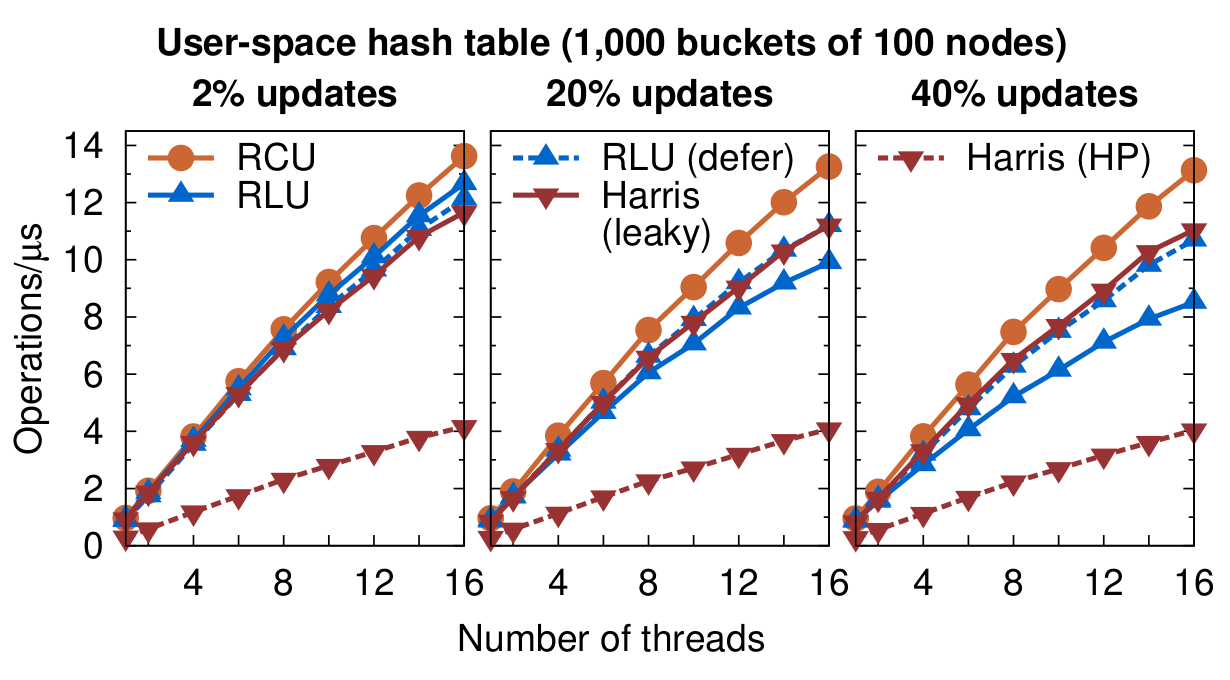
\includegraphics[width=0.8\textwidth]{user-space-hash-table-bench.png}
  \end{figure}

  \begin{itemize}
  \item buckets reduce W/W conflicts.
  \item basic RLU incurs visible penalties for increasing mutation ratios.\\
    $\rightarrow$ RLU synchronize calls that have more effect when operations
    are short and fast.
  \end{itemize}
  
\end{frame}

%=================================================================

\begin{frame}[t]
  \frametitle{Reference}
  \url{https://dl.acm.org/doi/10.1145/2815400.2815406}
\end{frame}

\end{document}
